% Filming 101 document for TinkerMill.
% Daniel Williams <dwilliams@port8080.net>

% Command for compiling:
% pdflatex Filming101 && pdflatex Filming101

% Use latexclasses/tmarticle if this is being included from the git as a
% submodule.
\documentclass[letterpaper]{latexclasses/tmarticle}

% Call the style file here.

% Some document info.
\renewcommand{\titleinfo}{Filming 101}

% Here's the document.
\begin{document}
\maketitle

\newpage
\tableofcontents

\newpage

\section{Camera}

\subsection{Preparing the Camera}

\begin{itemize}
    \item
    Charge the battery.
    
    Make sure that the battery is fully charged before filming.  Plug the camera
    in the night before to make sure you have a full charge.  The worst thing
    that can happen during filming is having the camera die during a shot.
    Another handy thing to have is a spare battery.  Also bring the charger
    along just incase there is power to use.

    \item
    Format the memory.
    
    Make sure to format the card before shooting.  The second worst thing that
    can happen is to run out of film, or rather empty space on the flash card.
    The most reliable formating method is to use the one build into the camera.
    This will ensure that the filesystem on the flash card is compatible with
    the camera.  Make sure to carry spares also.

    \item
    Recording settings.
    
    % Put something here about settings.

\end{itemize}

\subsection{Zooming}

\begin{itemize}
    \item
    Don't zoom if possible.
    
    Camera motion is one of the hardest things to master.  If it doesn't have to
    happen, don't do it.
    
    \item
    Prepare the zoom.
    
    Figure out where the zoom will start and stop.  Make sure to practice the
    zoom a number of times.  Any inconsistencies will be easily noticed.
    
    \item
    Dolly Zoom.
    
    Also known as the Alfred Hitchcock zoom, in this technique the camera is
    moved while zooming the opposite direction in order to keep the subject of
    the shot the same size while distorting the surrounding environment.
    
    \item
    Ken Burns Effect.
    
    Used heavily in documentaries, this technique adds motion to otherwise
    static material.  This includes zooming and panning to keep the audience
    engaged.  This is usually used when showing still images on screen during a
    talkover.

\end{itemize}

\subsection{Whitebalance}

% Explain white balance here.  Add photos comparing the [in]correct calibrtions.

\begin{itemize}
    \item
    Avoid Automatic.
    
    Most (if not all) cameras these days have automatic white balance.  If
    possible, don't use it.  Most of the time, it will get the color correction
    wrong.  The best option is to shoot in raw and handle the white balance in
    post production.
    
    \item
    Basic Settings.
    
    If raw shooting is not an option, which it usually isn't for filming, the
    easiest way to improve on the completely automatic method is to choose mode
    or hint for the whitebalance algorithm.  This hint is usually choosing the
    type of lighting (rough color temperature) of the scene.
    
    % Insert a pic of the various options here.
    
    \item
    Custom Adjustment.
    
    The best option for handling whitebalance is to use a custom setting.  Most
    cameras support setting the whitebalance adjustments by holding a white
    sheet of paper (should be a professionally collor calibrated gray card) in
    the view of the camera hand selecting a calibration function.  This should
    done in every location and even a few times throughout shooting, especially
    if shooting outdoors.
    
    % Insert picture of white sheet and clicking the calibration function.

\end{itemize}

\subsection{Basic Staging}

\begin{itemize}
    \item
    Wide shots.
    
    % Mark a stage for the subject.
    
    % Avoid crossing into that "stage" with the camera.
    
    % Avoid other, more interesting, subjects.
    
    \item
    Interviews.
    
    % Centering is boring.
    
    % Looking at the camera is creepy.
    
    \item
    Checking Lighting.
    
    % Not too bright, but bright enough.
    
    % Soft vs direct light.

\end{itemize}

\section{Editing}

\subsection{Importing onto the Computer}

% Which software should I demo?

\begin{itemize}

\end{itemize}

\subsection{Basic Editing}

\begin{itemize}
    \item
    The interface.
    
    Most non-linear video editing software packages use a somewhat standardized
    layout by default.  The layout consists of three major regions as
    demonstrated in figure 1..  The upper left quadrant contains the selection
    window.  The selection window is used to adjust setting and selections for
    clips in or being added to the filmstrip.  The upper right quadrant contains
    the preview window.  The preview window show the semi-compiled version of
    the final output at the selected frame of the filmstrip.  The lower two
    quadrants contain the filmstrip, which show the script of the project.  All
    clips, cuts, transitions, and other edits show up in the filmstrip.
    
    % Here's an example pic using the iMovie interface.  Probably should remake
    % using an opensource package interface.
    
    \begin{figure}[h]
        \centering
        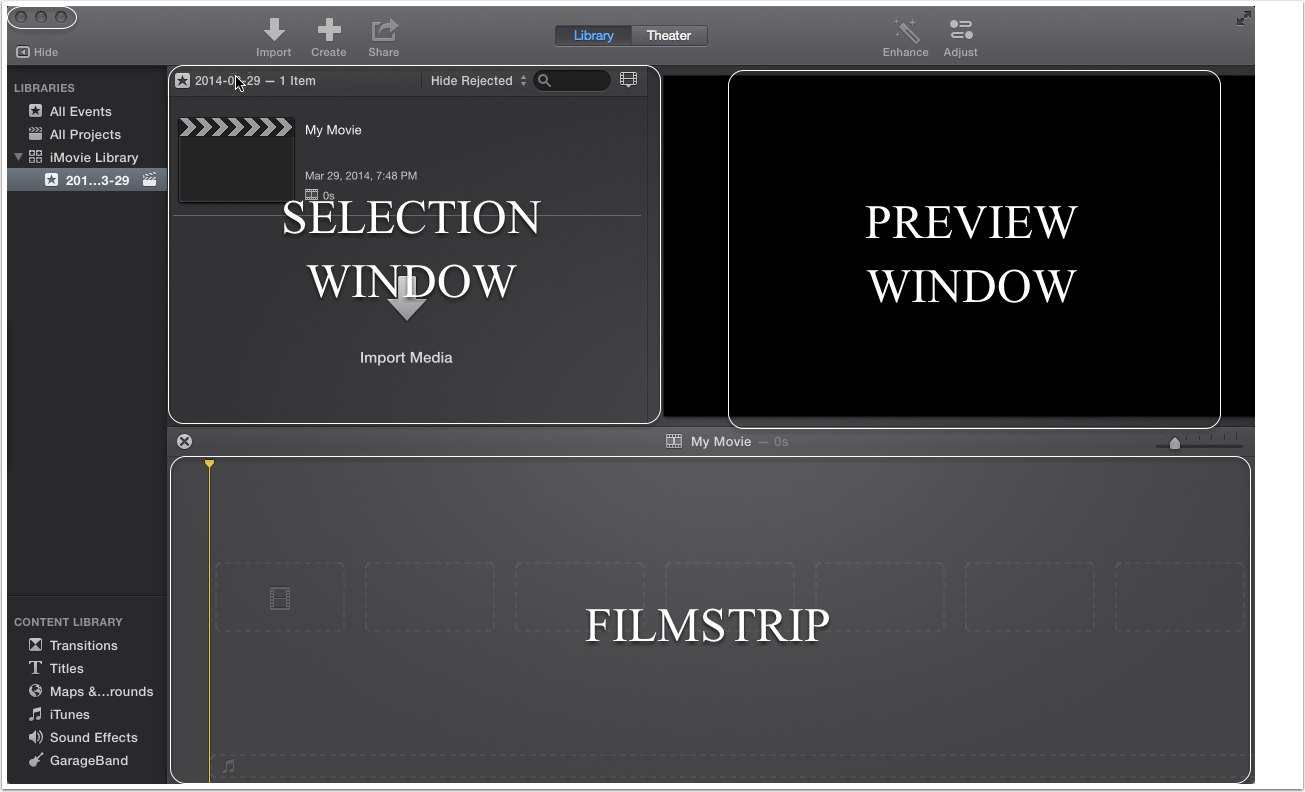
\includegraphics[width=6.0in]{iMovieInterface.png}
        \caption{Basic regions of non-linear editor interface.}
        % Add a reference here.
    \end{figure}
    
    \item
    Non-linear editing.
    
    % An explination of non-linear editing.
    
    \item
    Copy the files.
    
    % Copy to a scratch folder off the SD card.
    
    \item
    Open the project.
    
    \item
    Import the files.
    
    \item
    Adding clips to the filmstrip.
    
    % Dragging.
    
    % Trimming before adding.
    
    \item
    Transitions.
    
    % Cuts are the most used (lack of) transition.
    
    % Fades are good for starting and ending a scene.
    
    % Keep transitions short and simple.

\end{itemize}

\subsection{Sharing your Content}

\begin{itemize}
    \item
    Exporting.
    
    % What settings for which output (HD, DVD, Youtube)
    
    \item
    Uploading.
    
    % Howto blast your crap on youtube.

\end{itemize}

\end{document}
